\documentclass{beamer}

\mode<presentation> {
\usetheme{Madrid}
}

\usepackage{graphicx}
\usepackage{booktabs}

\title[Decision Tree]{Optimal binary decision tree}
\author{Mohammad Mahdi Heydari}
\institute[AUT] 
{
Amirkabir University of Technology \\ 
\medskip
\textit{} 
}
\date{June 1, 2019} 

\begin{document}

\begin{frame}
\titlepage 
\end{frame}

\begin{frame}
\frametitle{Overview}
\tableofcontents
\end{frame}

\section{Introduction}
\begin{frame}
	\frametitle{Introduction}
	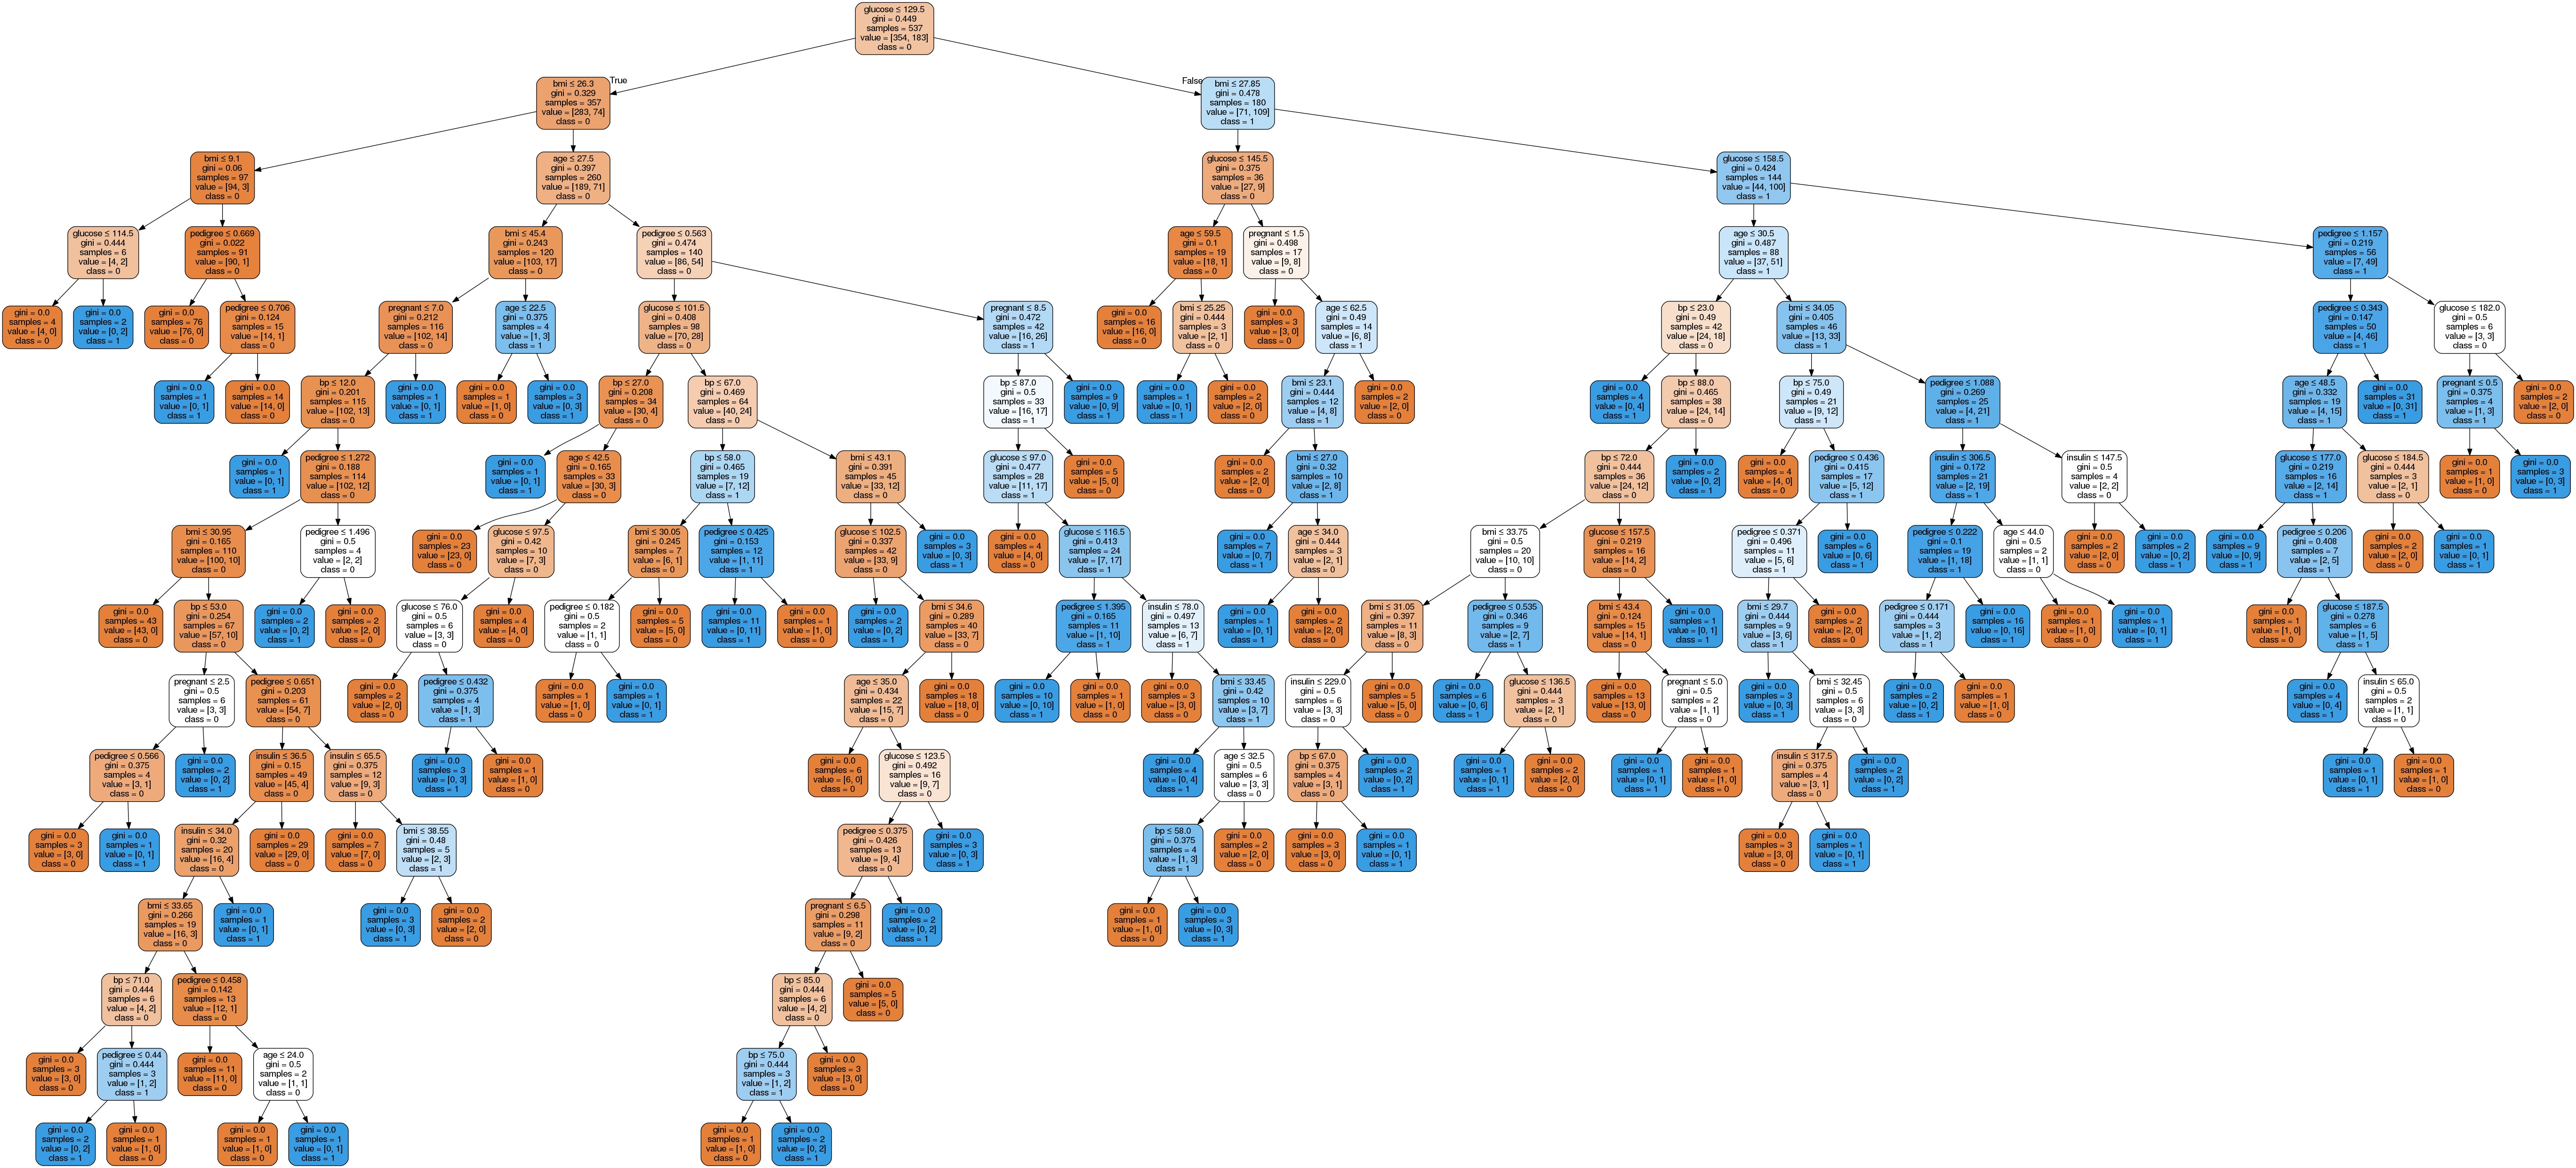
\includegraphics[width=\linewidth]{Pics/dtree.jpg}
\end{frame}

\begin{frame}
	\frametitle{Introduction}
	\begin{itemize}
	\item
	An optimal binary decision tree is one which minimizes the expected number of tests required to identify the unknown object.	
	\item
	Large amount of effort had been put into finding efficient algorithms for constructing optimal binary decision tree.
	\item
	On supposition that $P \ne NP$, such algorithm does not exist. 
	\item
	It supplies motivation for finding efficient heuristics for constructing near-optimal decision trees.
	\end{itemize}
\end{frame}

\begin{frame}[fragile]
\frametitle{Definition}
	\begin{block}{Sets}
		Let $X=\{x_1, ..., x_n\}$ be a finite set of objects and let $\tau=\{T_1, ..., T_t \}$ be a finite set of tests.
		for each test $T_i$, $1\le i \le t$ and object $x_j$, $1 \le j \le n$, we either have $T_i(x_j)= true$ or $T_i(x_j)= false $.
		$T_i$ also denotes the set $\{x \in X | T_i(x) = true \}$.
	\end{block}

	\begin{block}{Problem}
		The problem is to construct an identification procedure for the objects in $X$ such that the expected number of tests
		required to completely identify an element of X is minimal. At each non-terminal node, a test is specified and terminal
		nodes specify objects in $X$.
	\end{block}
\end{frame}

\begin{frame}[fragile]
\frametitle{Definition}
	\begin{block}{Procedure}
		To apply the identification procedure one first applies the test specified at the root to the unknown object; if it
		is false one takes the left branch, otherwise the right. This procedure is repeated at the root of each successive subtree until one reaches a terminal node which names the unknown object.
	\end{block}

	\begin{block}{Cost}
		Let $p(x_i)$ be the length of the path from the root to the terminal node naming $x_i$, that is, the number of tests
		required to identify $x_i$. Then the cost of this tree will be:
		\[ \sum_{x_i \in X} p(x_i) \]
	\end{block}
\end{frame}

\begin{frame}
	\frametitle{Optimization vs. Decision}
	\begin{figure}
		
\includegraphics[height=0.33\textheight]{Pics/opt.jpg}
	\end{figure}
	
	\begin{figure}
		
\includegraphics[height=0.3\textheight]{Pics/decision.png}
	\end{figure}
\end{frame}

\section{Decision Problem}
\begin{frame}
	\frametitle{Decision Problem}
	\begin{block}{Decision}
		The decision tree problem $DT(\tau, X, w)$ is to determine whether there exists a decision tree with 
		cost less than or equal to $w$ given $\tau$ and $X$.
	\end{block}
	\begin{theorem}
		$DT(\tau, X, w)$ is NP-complete.
	\end{theorem}
	\begin{proof}
		$DT\in NP$. since a a non-deterministic Turing machine can guess the decision tree and then see if its
		weight is less than or equal to $w$.
	\end{proof}
\end{frame}

\begin{frame}
	\frametitle{Decision Problem}
	\begin{proof}
		To show that DT is NP-complete, we show that $EC3 \alpha DT$, where EC3 is the problem of finding
		an exact cover for a set X, and where each of the subsets available for use contains exactly 3 elements.
		More precisely, we are given a set $X={x_1,... , x_n}$ and a family $\tau = {T_1,... , T_t}$ of subsets
		of X, such that $|T_i|=3$ for $1\le i \le t$, and we wish to find a subset $S$ of $\tau$ such that
		$\bigcup\limits_{T_i \in S} T_{i} = X$ and $(({T_i, T_j}\subseteq S$ and 
		$i\ne j) \Rightarrow T_i \cap T_j = \emptyset)$. The exact cover problem EC (where there is no restriction on the size of each $T_i$) is known to be NP-complete. To show that EC3 is NP-complete,
		we show $3DM \alpha EC3$, where 3DM is the problem of finding a "three-dimensional matching".
	\end{proof}
\end{frame}

\section{Approximation DT}
\begin{frame}
	\frametitle{Approximation DT}
	Given a set of binary m-bit strings S, choosing some bit i always partitions the items into two sets $S_0$ and $S_1$ where $S_0$ contains those items with bit i = 0 and $S_1$ contains those items with i = 1. A greedy strategy
	for splitting a set S chooses the bit i which minimizes the difference between the size of $S_0$ and $S_1$. In other
	words, it chooses the bit which most evenly partitions the set. Using this strategy, consider the following
	greedy algorithm for constructing decision trees of the DT type given a set of n items X:
\end{frame}	

\begin{frame}
	\frametitle{Approximation DT}
	\begin{figure}
		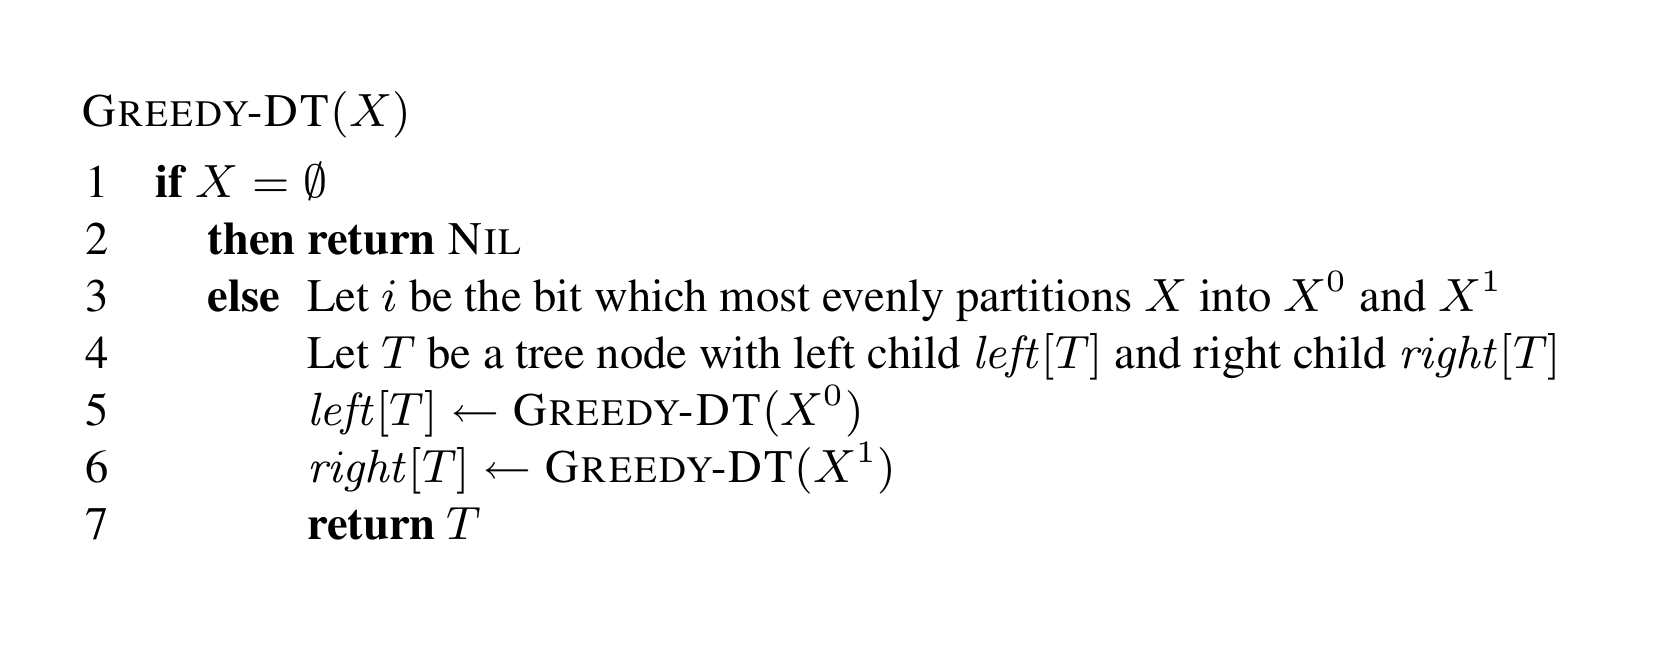
\includegraphics[width=0.9\linewidth]{Pics/greedy.png}
	\end{figure}
	
	A straightforward implementation on this algorithm runs in time $O(mn^2)$. While the algorithm does not
	always give an optimal solution, it does approximate it within a factor of $ln(n) + 1$.
\end{frame}

\section{Application}
\begin{frame}
	\frametitle{Application}
	\begin{block}{}
		In some applications we have X set as tuples with some attributes and we are free to choose $\tau$ set.
		The leaves should only classify $x_j$s (vs. identification).
		There are some greedy algorithms to construct these decision trees. Our goal will be to find a 
		split leading to the most monotonous subtrees.
	\end{block}
\end{frame}
\begin{frame}
	\frametitle{Create Test Set}
	Split Approaches:
	\begin{itemize}
		\item
		Oblique
		\item
		Axis-Parallel \checkmark
	\end{itemize}
	\begin{figure}
		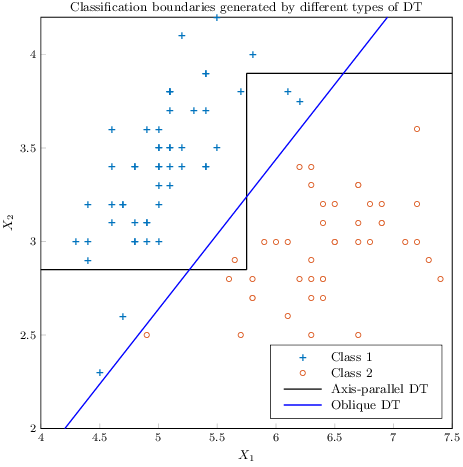
\includegraphics[width=0.5\linewidth]{Pics/oblique.png}
	\end{figure}
\end{frame}

\begin{frame}
	\frametitle{Split Measures}
	\begin{itemize}
		\item Information Gain
		\[Info(D)=-\sum_{i=1}^{m} p_i\hspace{4pt} log_2 (p_i)\]
		\[Info_A(D)= \sum_{j=1}^{v} \frac{|D_j|}{|D|}\times Info(D_j)\]
		\[Gain(A) = Info(D) - Info_A(D) \]
		
		\item Gini (only binary)
		\[Gini(D) = 1- \sum_{i=1}^{m} p_i^2\]
		\[Gini_A(D) = \frac{|D_1|}{|D|}Gini(D_1) + \frac{|D_2|}{|D|}Gini(D_2)\]
		\[\Delta Gini(A) = Gini(D) - Gini_A(D)\]
	\end{itemize}
\end{frame}

\begin{frame}
	\frametitle{References}
	\begin{itemize}
		\item
		Hyafil, Laurent \& L. Rivest, Ronald. (1976). Constructing Optimal Binary Decision Trees is NP-Complete. Inf. Process. Lett.. 5. 15-17. 10.1016/0020-0190(76)90095-8. 
		\item
		Adler, Micah \& Heeringa, Brent. (2008). Approximating Optimal Binary Decision Trees. 10.1007/978-3-540-85363-3\_1. 
		\item
		Data Mining: Concepts and Techniques, Second Edition
		Jiawei Han and Micheline Kamber (2006)
	\end{itemize}
\end{frame}

\begin{frame}
	\Huge
	\centering
	Any Question?
\end{frame}

\end{document} 